\documentclass[]{article}
\usepackage[T1]{fontenc}
\usepackage{lmodern}
\usepackage{amssymb,amsmath}
\usepackage{ifxetex,ifluatex}
\usepackage{fixltx2e} % provides \textsubscript
% use upquote if available, for straight quotes in verbatim environments
\IfFileExists{upquote.sty}{\usepackage{upquote}}{}
\ifnum 0\ifxetex 1\fi\ifluatex 1\fi=0 % if pdftex
  \usepackage[utf8]{inputenc}
\else % if luatex or xelatex
  \ifxetex
    \usepackage{mathspec}
    \usepackage{xltxtra,xunicode}
  \else
    \usepackage{fontspec}
  \fi
  \defaultfontfeatures{Mapping=tex-text,Scale=MatchLowercase}
  \newcommand{\euro}{€}
\fi
% use microtype if available
\IfFileExists{microtype.sty}{\usepackage{microtype}}{}
\usepackage{graphicx}
% Redefine \includegraphics so that, unless explicit options are
% given, the image width will not exceed the width of the page.
% Images get their normal width if they fit onto the page, but
% are scaled down if they would overflow the margins.
\makeatletter
\def\ScaleIfNeeded{%
  \ifdim\Gin@nat@width>\linewidth
    \linewidth
  \else
    \Gin@nat@width
  \fi
}
\makeatother
\let\Oldincludegraphics\includegraphics
{%
 \catcode`\@=11\relax%
 \gdef\includegraphics{\@ifnextchar[{\Oldincludegraphics}{\Oldincludegraphics[width=\ScaleIfNeeded]}}%
}%
\ifxetex
  \usepackage[setpagesize=false, % page size defined by xetex
              unicode=false, % unicode breaks when used with xetex
              xetex]{hyperref}
\else
  \usepackage[unicode=true]{hyperref}
\fi
\hypersetup{breaklinks=true,
            bookmarks=true,
            pdfauthor={},
            pdftitle={JINR PAC руководство},
            colorlinks=true,
            citecolor=blue,
            urlcolor=blue,
            linkcolor=magenta,
            pdfborder={0 0 0}}
\urlstyle{same}  % don't use monospace font for urls
\setlength{\parindent}{0pt}
\setlength{\parskip}{6pt plus 2pt minus 1pt}
\setlength{\emergencystretch}{3em}  % prevent overfull lines
\setcounter{secnumdepth}{0}

\title{JINR PAC руководство}
\author{}
\date{Декабрь 17, 2018}

\begin{document}
\maketitle

\section{Основы работы спектрометра JINR PAC}

Таким образом при первоначальном включении спектрометра необходимо
выполнить следующие процедуры для запуска накопления:

\begin{enumerate}
\def\labelenumi{\arabic{enumi}.}
\item
  \hyperref[firmwareux5fFPGA]{Загрузить прошивку в ПЛИС}
\item
  \hyperref[firmwareux5fUSB]{Загрузить прошивку в USB контроллер}
\item
  \hyperref[initux5fFPGA]{Провести инициализацию параметров ПЛИС}
\item
  \hyperref[setux5fexposition]{Задать параметры экспозиции}
\item
  \hyperref[startux5fexposition]{Провести запуск экспозиции}
\end{enumerate}

В том случае, если питание спектрометра не выключалось и процедуры
прошивки и инициализации были выполнены ранее, то первые три пункта
этого руководства можно пропустить.

\section{Загрузка прошивки в ПЛИС}

Загрузка прошивки в ПЛИС из ОС Windows XP

\begin{enumerate}
\def\labelenumi{\arabic{enumi}.}
\item
  Запустите программу Impact
\item
  Кликните дважды по Boundary Scan в окне программы в левом верхнем меню

  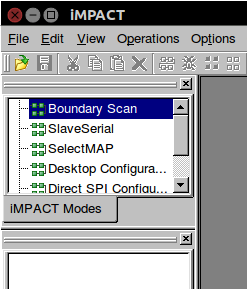
\includegraphics{./imgs/firmware_FPGA_win_Bounddary_Scan.png}
\item
  Кликните правой кнопкой мыши для добавления устройства в поле Boundary
  Scan справа
\item
  Выберите Initialize chain

  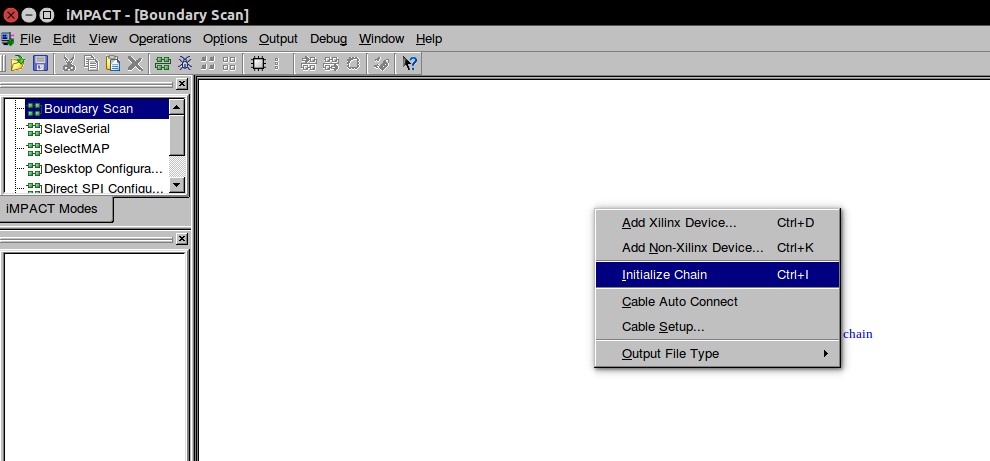
\includegraphics{./imgs/firmware_FPGA_win_Add_device.png}
\item
  Выберите прошивку ПЛИС

  Одна из рабочих версий прошивки находится по адресу

\begin{verbatim}
          E:/work/Proshivki/9253/Right/4poroga+count.bit
        
\end{verbatim}

  В открывшемся окне кликните Ok
\item
  Кликните правой кнопкой мыши на устройстве и выберите Program...

  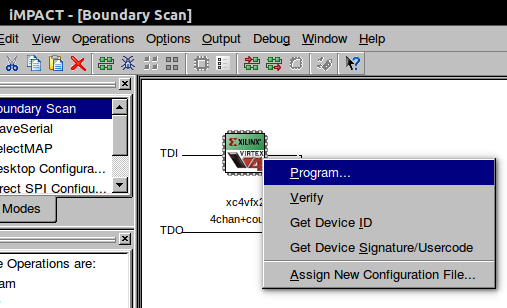
\includegraphics{./imgs/firmware_FPGA_win_Program.png}
\item
  В появившемся окне кликните Ok. После нескольких секунд прошивка ПЛИС
  будет завершена и в поле Boundary Scan появится надпись на синем фоне
  Program Succeded
\item
  На этом процедура прошивки ПЛИС завершена. Программу Impact можно
  закрывать. Сохранять проект не надо.
\end{enumerate}

Загрузка прошивки из ОС Linux

\begin{enumerate}
\def\labelenumi{\arabic{enumi}.}
\item
  Запустите Terminal
\item
  Перейдите в каталог с пакетом програм Xilinx ISE:

\begin{verbatim}
          cd ~/job/xilinx_soft/bin
        
\end{verbatim}
\item
  Запустите программу impact:

\begin{verbatim}
          impact
        
\end{verbatim}
\item
  Далее последовательность действий
  \hyperref[uploadux5ffirmwareux5fFPGAux5fwin]{такая же как в Windows
  XP}. Иногда может потребоваться произвести поиск ПЛИС () два раза
  и/или переподключить USB кабель программатора ПЛИС к ПК.
\end{enumerate}

\section{Загрузка прошивки в USB контроллер}

Загрузка прошивки из OC Linux (с использованием графического
интерфейса):

\begin{enumerate}
\def\labelenumi{\arabic{enumi}.}
\item
  Запустите Terminal
\item
  Запустите программу Cypress USB control center набрав в Терминале
  команду:

\begin{verbatim}
          cyusb_linux
        
\end{verbatim}

  и затем нажмите клавишу Enter
\item
  В Cypress USB control center выберите необходимый контроллер. Он
  должен иметь VID=04b4 и PID=8613

  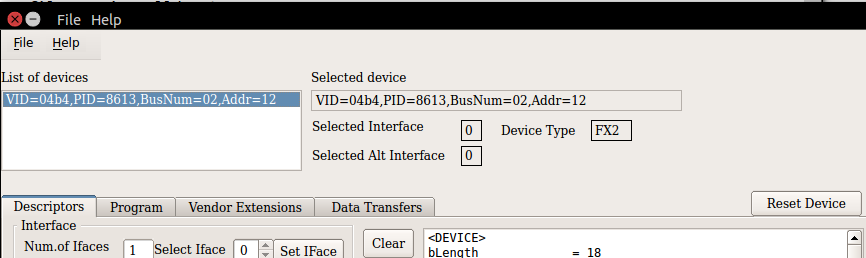
\includegraphics{./imgs/firmware_USB_lin_Select_controller.png}
\item
  Выберите вкладку Program, владку FX2. Затем в списке Download to
  -\textgreater{} выберите пункт RAM, в списке Which RAM выберите пункт
  Internal

  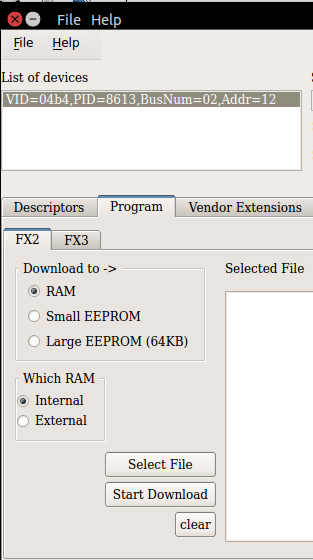
\includegraphics{./imgs/firmware_USB_lin_Select_RAM.png}
\item
  Нажмите на кнопку Select File и выберите необходимую прошивку USB
  контроллера

  Одна из рабочих прошивок находится по адресу:

\begin{verbatim}
          /home/das/job/dsp/firmwares/512x4.hex
        
\end{verbatim}
\item
  Произведите загрузку прошивки в контроллер нажатием кнопки Start
  Download

  В случае успешной прошивки появится диалоговое окно с текстом
  "Successfully downloaded"

  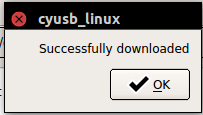
\includegraphics{./imgs/firmware_USB_lin_Success.png}

  В случае возникновения ошибки подробности об ошибке могут быть
  прочитаны в окне Терминала
\item
  После прошивки контроллер необходимо перезагрузить путем нажатия
  кнопки Reset Device в программе cyusb\_linux

  При этом PID контроллера в списке List of devices должен измениться и
  стать PID=00f1 (VID остается прежним)
\end{enumerate}

Загрузка прошивки из OC Linux (с использованием интерфейса терминала):

\begin{enumerate}
\def\labelenumi{\arabic{enumi}.}
\item
  Откройте Terminal
\item
  В терминале наберите следующую команду:

\begin{verbatim}
      download_fx2 ...
    
\end{verbatim}

  Эта команда запускает программу download\_fx2, которая загружает
  прошивку 512x4.hex в USB контроллер с VID=04b4 и PID=8613
\end{enumerate}

\section{Инициализация параметров ПЛИС}

\begin{enumerate}
\def\labelenumi{\arabic{enumi}.}
\item
  Запустите Terminal
\item
  Запустите программу dsppac набрав в Терминале команду:

\begin{verbatim}
           dsppac
         
\end{verbatim}

  и затем нажмите клавишу Enter
\item
  Для настройки параметров ПЛИС выберите в верхнем меню программы
  ExpositionMode -\textgreater{} Settings

  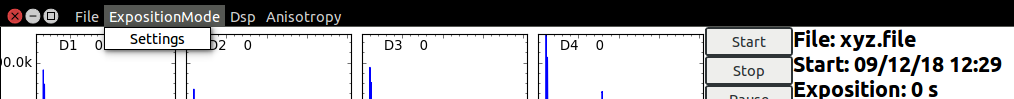
\includegraphics{./imgs/set_FPGA_Select_menu.png}
\item
  В появившемся окне выставите значения порога для каждого из четырех
  детекторов и напротив полей с порогами нажмите кнопку Set porog

  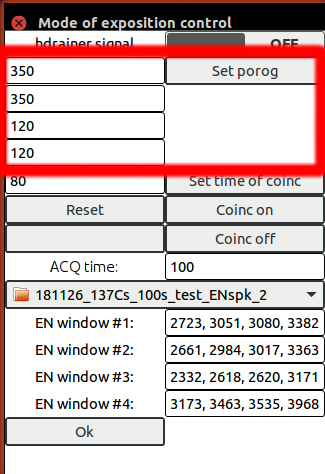
\includegraphics{./imgs/set_FPGA_Set_porog.png}
\item
  Выставите значение времени совпадений и напротив соответствующего поля
  нажмите кнопку Set time of coinc. После этого нажмите кнопку Reset

  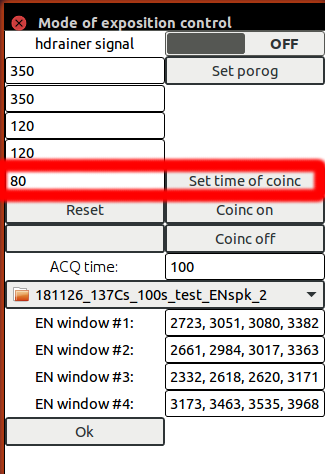
\includegraphics{./imgs/set_FPGA_Set_timeofcoinc.png}
\item
  Для выбора режима накопления с совпадениями или без совпадений нажмите
  кнопку Coinc on или Coinc off, соответственно. После этого нажмите
  кнопку Reset.

  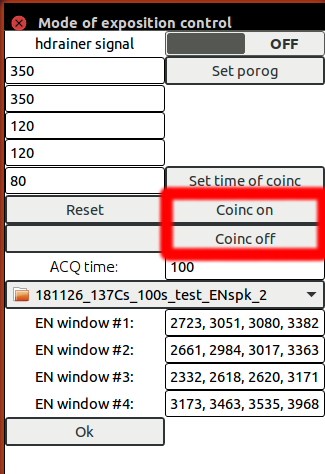
\includegraphics{./imgs/set_FPGA_Coinc_mode.png}
\end{enumerate}

\section{Установка параметров экспозиции}

\begin{enumerate}
\def\labelenumi{\arabic{enumi}.}
\item
  Запустите Terminal и из него запустите программу dsppac
\item
  Для установки параметров экспозиции выберите в верхнем меню программы
  ExpositionMode -\textgreater{} Settings

  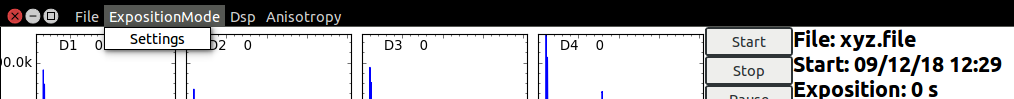
\includegraphics{./imgs/set_FPGA_Select_menu.png}
\item
  В появившемся списке вы можете задать такие параметры экспозиции, как

  \begin{itemize}
  \item
    Сохранять ли накопленные формы сигналов с помощью
    ползунка-переключателя hdrainer signal OFF/ON (по умолчанию OFF)
  \item
    Время экспозиции (накопления) в поле ACQ time

    В том случае если в этом поле указано целое число, то оно
    интерпретируется, как время в секундах.

    Также возможны следующие форматы указания времени: "123m", "123h",
    "123d" -, которые задают время экспозиции в минутах (minutes), часах
    (hours), днях (days), соответственно.
  \item
    Каталог, в котором будут сохраняться накопленные спектры
  \item
    Энергетические окна для каждого из четырех детекторов в полях EN
    window \#1-4 в формате

    "g1\_l, g1\_r, g2\_l, g2\_r", где

    g1\_l - целое число, соответствующее \emph{левой} границе
    энергетического окна для гамма-кванта \emph{1} в каскаде

    g1\_r - целое число, соответствующее \emph{правой} границе
    энергетического окна для гамма-кванта \emph{1} в каскаде

    g2\_l - целое число, соответствующее \emph{левой} границе
    энергетического окна для гамма-кванта \emph{2} в каскаде

    g2\_r - целое число, соответствующее \emph{правой} границе
    энергетического окна для гамма-кванта \emph{2} в каскаде

    Все энергетические окна задаются в каналах энергетического спектра.
  \end{itemize}
\end{enumerate}

\section{Запуск экспозиции}

\begin{enumerate}
\def\labelenumi{\arabic{enumi}.}
\item
  Запустите Terminal и из него запустите программу dsppac
\item
  Для запуска экпозиции нажмите кнопку Start в основном окне программы.
  При этом при накоплении эта кнопка окажется вдавленной. Для остановки
  нажмите кнопку Stop.

  При нормальном запуске экспозиции в поле Time будет отображаться время
  с начала экспозиции и в поле Intensity интенсивность со всех четырех
  детекторов (в режиме совпадений или без).

  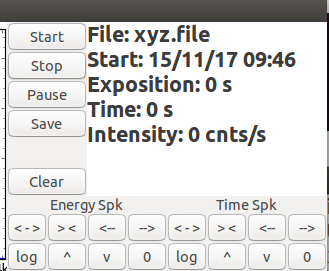
\includegraphics{./imgs/start_exposition_Btns_Info_field.png}
\end{enumerate}

\end{document}
